\documentclass{article}
\usepackage{graphicx}
\usepackage{subcaption}
\usepackage{booktabs}
\usepackage{array}
\usepackage{geometry}
\geometry{margin=1in}
\usepackage{amsmath}
\usepackage{booktabs}

\begin{document}

\begin{figure}[ht]
  \centering
  \begin{subfigure}{0.3\textwidth}
    \centering
    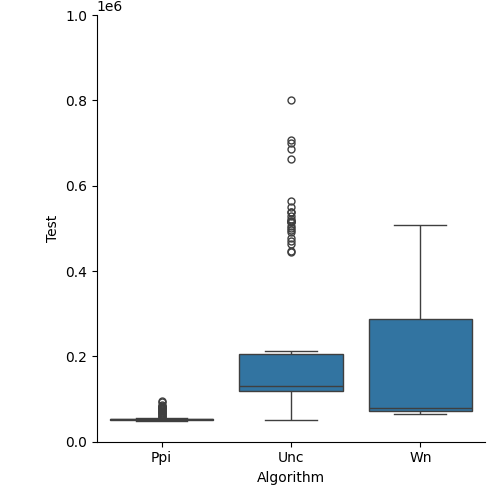
\includegraphics[width=\linewidth]{../figureIntRandom100.png}
    \caption{Size: 100}
    \label{fig:img1}
  \end{subfigure}
  \begin{subfigure}{0.3\textwidth}
    \centering
    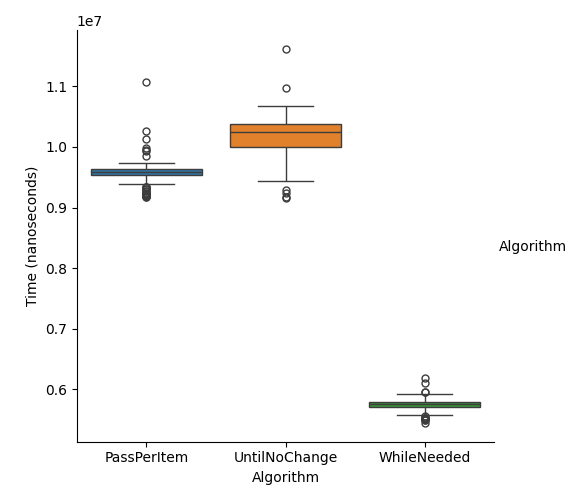
\includegraphics[width=\linewidth]{../figureIntRandom1000.png}
    \caption{Size 1000}
    \label{fig:img2}
  \end{subfigure}
  \begin{subfigure}{0.3\textwidth}
    \centering
    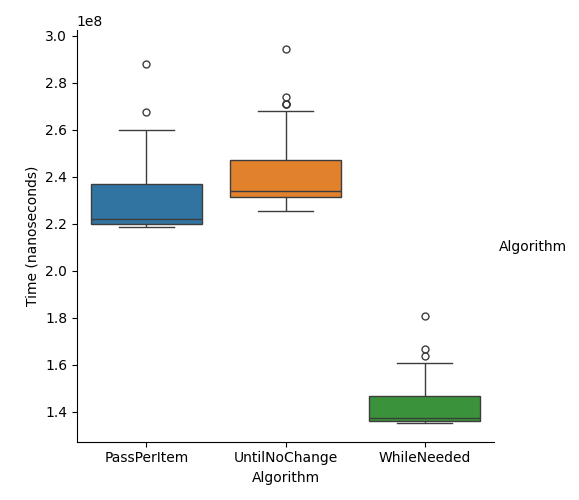
\includegraphics[width=\linewidth]{../figureIntRandom5000.png}
    \caption{Size 5000}
    \label{fig:img3}
  \end{subfigure}
  \caption{Time to sort array of random Integers}
  \label{fig:three_images}
\end{figure}

\begin{figure}[ht]
  \centering
  \begin{subfigure}{0.3\textwidth}
    \centering
    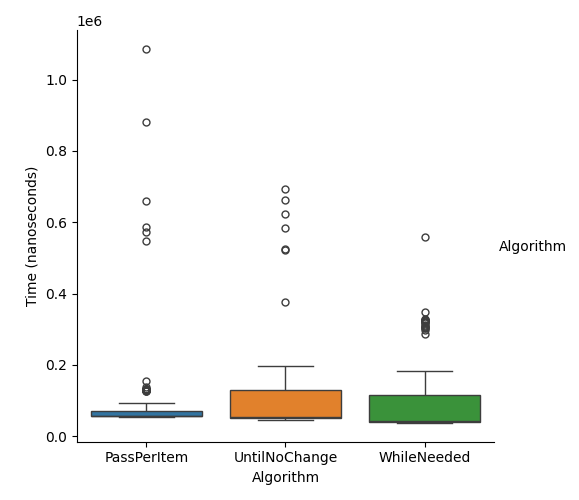
\includegraphics[width=\linewidth]{../figureByteRandom100.png}
    \caption{Size: 100}
    \label{fig:img1}
  \end{subfigure}
  \begin{subfigure}{0.3\textwidth}
    \centering
    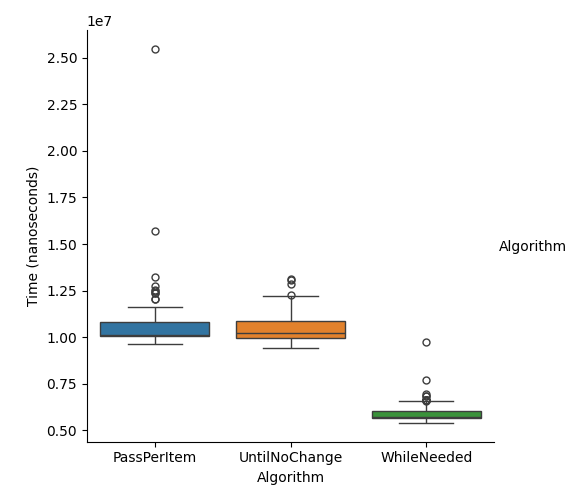
\includegraphics[width=\linewidth]{../figureByteRandom1000.png}
    \caption{Size 1000}
    \label{fig:img2}
  \end{subfigure}
  \begin{subfigure}{0.3\textwidth}
    \centering
    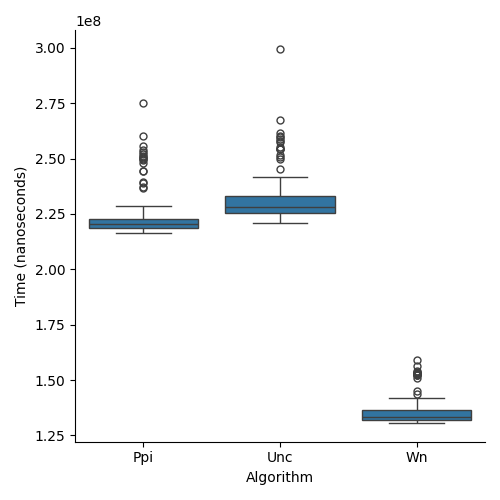
\includegraphics[width=\linewidth]{../figureByteRandom5000.png}
    \caption{Size 5000}
    \label{fig:img3}
  \end{subfigure}
  \caption{Time to sort random array of Bytes}
  \label{fig:three_images}
\end{figure}

\begin{figure}[ht]
  \centering
  \begin{subfigure}{0.3\textwidth}
    \centering
    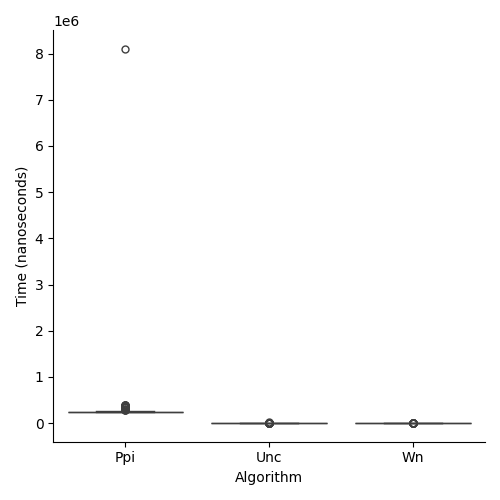
\includegraphics[width=\linewidth]{../figureStringRandom100.png}
    \caption{Size: 100}
    \label{fig:img1}
  \end{subfigure}
  \begin{subfigure}{0.3\textwidth}
    \centering
    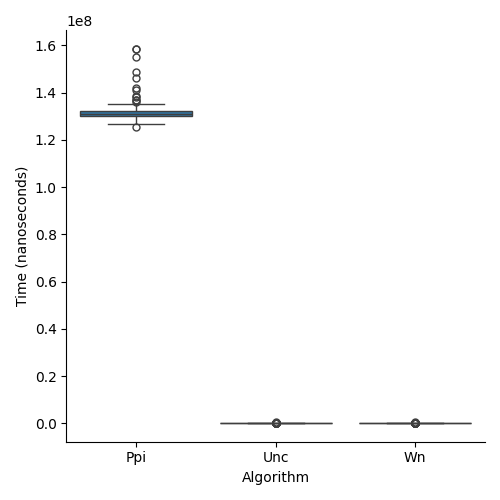
\includegraphics[width=\linewidth]{../figureStringRandom1000.png}
    \caption{Size 1000}
    \label{fig:img2}
  \end{subfigure}
  \begin{subfigure}{0.3\textwidth}
    \centering
    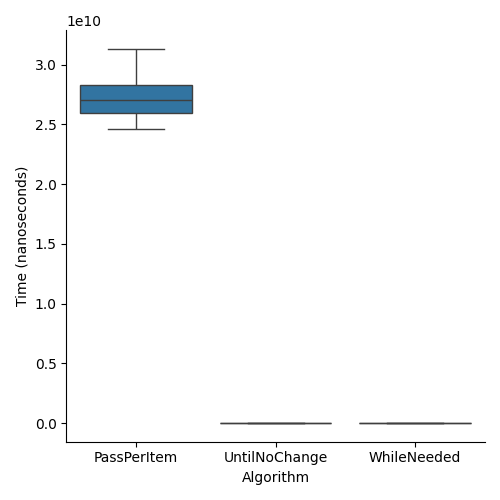
\includegraphics[width=\linewidth]{../figureStringRandom5000.png}
    \caption{Size 5000}
    \label{fig:img3}
  \end{subfigure}
  \caption{Time to sort random array of String}
  \label{fig:three_images}
\end{figure}

\begin{table}[htbp]
    \centering
    \begin{tabular}{ccrrrrr}
        \toprule
        \textbf{Size} & \textbf{Algorithm} & \textbf{Minimum} & \textbf{First Quartile} & \textbf{Median} & \textbf{Third Quartile} & \textbf{Maximum} \\
        \midrule
        100 & PassPerItem & 49.85 & 50.07 & 50.31 & 50.82 & 87.38 \\
        100 & UntilNoChange & 56.74 & 56.92 & 57.06 & 57.45 & 103.16 \\
        100 & WhileNeeded & 33.44 & 33.50 & 33.59 & 33.78 & 69.36 \\
        1000 & PassPerItem & 9'606.17 & 9'640.39 & 9'665.68 & 9'751.96 & 31'493.50 \\
        1000 & UntilNoChange & 9'548.54 & 9'562.60 & 9'575.98 & 9'774.66 & 31'540.57 \\
        1000 & WhileNeeded & 5'481.91 & 5'497.36 & 5'507.04 & 5'569.73 & 17'908.92 \\
        5000 & PassPerItem & 20'8339.31 & 210'349.57 & 212'377.40 & 219'466.91 & 263'363.72 \\
        5000 & UntilNoChange & 210'984.56 & 211'619.51 & 214'544.31 & 227'371.03 & 298'996.13 \\
        5000 & WhileNeeded & 122'377.71 & 122'787.50 & 124'621.14 & 132'163.16 & 173'597.92 \\
        \bottomrule
    \end{tabular}
    \caption{Performance Metrics for arrays of Descending Integers (in microseconds)}
    \label{tab:performance}
\end{table}

\begin{table}[htbp]
    \centering
    \begin{tabular}{ccrrrrr}
        \toprule
        \textbf{Size} & \textbf{Algorithm} & \textbf{Minimum} & \textbf{First Quartile} & \textbf{Median} & \textbf{Third Quartile} & \textbf{Maximum} \\
        \midrule
        100 & PassPerItem & 58.54 & 58.77 & 58.96 & 59.42 & 99.76 \\
        100 & UntilNoChange & 57.71 & 58.16 & 58.32 & 58.76 & 104.34 \\
        100 & WhileNeeded & 42.91 & 43.02 & 43.13 & 43.43 & 75.81 \\
        1000 & PassPerItem & 9'548.90 & 9'708.79 & 9'747.38 & 9'877.97 & 17'988.70 \\
        1000 & UntilNoChange & 9'859.16 & 10'082.39 & 10'124.00 & 10'387.20 & 17'207.29 \\
        1000 & WhileNeeded & 5'687.05 & 5'857.50 & 5'881.01 & 5'975.96 & 14'572.42 \\
        5000 & PassPerItem & 205'850.43 & 209'231.70 & 211'795.54 & 214'074.12 & 241'904.37 \\
        5000 & UntilNoChange & 215'364.05 & 216'803.60 & 219'137.71 & 222'237.53 & 249'848.90 \\
        5000 & WhileNeeded & 123'721.80 & 125'714.37 & 126'542.95 & 129'139.10 & 151'971.81 \\
        \bottomrule
    \end{tabular}
    \caption{Performance Metrics for arrays of Descending Bytes(in microseconds)}
    \label{tab:performance_2}
\end{table}

\begin{table}[htbp]
    \centering
    \begin{tabular}{ccrrrrr}
        \toprule
        \textbf{Size} & \textbf{Algorithm} & \textbf{Minimum} & \textbf{First Quartile} & \textbf{Median} & \textbf{Third Quartile} & \textbf{Maximum} \\
        \midrule
        100 & PassPerItem & 250.51 & 260.69 & 262.30 & 264.39 & 361.71 \\
        100 & UntilNoChange & 252.84 & 264.19 & 265.84 & 268.57 & 300.53 \\
        100 & WhileNeeded & 121.71 & 126.99 & 127.92 & 129.11 & 158.24 \\
        1000 & PassPerItem & 117'837.06 & 119'357.54 & 121'274.97 & 123'099.46 & 143'828.36 \\
        1000 & UntilNoChange & 117'809.62 & 119'980.49 & 121'655.67 & 123'569.40 & 140'236.91 \\
        1000 & WhileNeeded & 45'292.69 & 45'868.37 & 46'430.09 & 47'424.17 & 57'093.29 \\
        5000 & PassPerItem & 25'781'857.71 & 26'383'544.20 & 26'828'103.50 & 27'380'123.07 & 29'426'932.85 \\
        5000 & UntilNoChange & 25'842'208.87 & 26'413'720.27 & 26'818'579.97 & 27'416'407.67 & 29'207'443.63 \\
        5000 & WhileNeeded & 8'228'578.19 & 8'406'592.12 & 8'543'826.54 & 8'635'735.72 & 9'775'953.45 \\
        \bottomrule
    \end{tabular}
    \caption{Performance Metrics for arrays of Descending Strings(in microseconds)}
    \label{tab:performance_4}
\end{table}

\begin{table}[htbp]
    \centering
    \begin{tabular}{ccrrrrr}
        \toprule
        \textbf{Size} & \textbf{Algorithm} & \textbf{Minimum} & \textbf{First Quartile} & \textbf{Median} & \textbf{Third Quartile} & \textbf{Maximum} \\
        \midrule
        100 & PassPerItem & 31.47 & 31.64 & 31.71 & 31.84 & 47.30 \\
        100 & UntilNoChange & 0.46 & 0.51 & 0.53 & 0.55 & 1.28 \\
        100 & WhileNeeded & 0.42 & 0.47 & 0.49 & 0.50 & 1.05 \\
        1000 & PassPerItem & 7'913.74 & 7'981.70 & 8'007.96 & 8'041.87 & 8261.34 \\
        1000 & UntilNoChange & 8.72 & 8.83 & 8.95 & 9.11 & 13.34 \\
        1000 & WhileNeeded & 8.60 & 8.72 & 8.78 & 8.97 & 10.79 \\
        5000 & PassPerItem & 172'160.11 & 172'462.95 & 175'633.39 & 179'902.05 & 223'133.42 \\
        5000 & UntilNoChange & 37.61 & 37.76 & 37.99 & 39.33 & 46.91 \\
        5000 & WhileNeeded & 37.06 & 37.18 & 37.39 & 38.58 & 69.91 \\
        \bottomrule
    \end{tabular}
    \caption{Performance Metrics for array of Ascending Integers (in microseconds)}
    \label{tab:performance_5}
\end{table}

\begin{table}[htbp]
    \centering
    \begin{tabular}{ccrrrrr}
        \toprule
        \textbf{Size} & \textbf{Algorithm} & \textbf{Minimum} & \textbf{First Quartile} & \textbf{Median} & \textbf{Third Quartile} & \textbf{Maximum} \\
        \midrule
        100 & PassPerItem & 33.12 & 33.17 & 33.22 & 39.41 & 61.92 \\
        100 & UntilNoChange & 0.39 & 0.41 & 0.44 & 0.65 & 1.10 \\
        100 & WhileNeeded & 0.42 & 0.46 & 0.50 & 0.65 & 1.09 \\
        1000 & PassPerItem & 7'829.75 & 7'881.66 & 7'900.80 & 8'243.30 & 14'010.38 \\
        1000 & UntilNoChange & 8.63 & 8.81 & 8.91 & 9.25 & 16.23 \\
        1000 & WhileNeeded & 8.51 & 8.67 & 8.79 & 9.12 & 16.05 \\
        5000 & PassPerItem & 170'007.62 & 17'1708.70 & 173'837.23 & 179'121.64 & 200'752.12 \\
        5000 & UntilNoChange & 36.90 & 37.19 & 38.38 & 39.96 & 43.44 \\
        5000 & WhileNeeded & 36.48 & 36.74 & 37.92 & 39.49 & 44.25 \\
        \bottomrule
    \end{tabular}
    \caption{Performance Metrics for array of Ascending Bytes (in microseconds)}
    \label{tab:performance_6}
\end{table}

\begin{table}[htbp]
    \centering
    \begin{tabular}{ccrrrrr}
        \toprule
        \textbf{Size} & \textbf{Algorithm} & \textbf{Minimum} & \textbf{First Quartile} & \textbf{Median} & \textbf{Third Quartile} & \textbf{Maximum} \\
        \midrule
        100 & PassPerItem & 2'344.88 & 2'370.67 & 2'390.62 & 2'451.50 & 3925.87 \\
        100 & UntilNoChange & 2.70 & 2.78 & 2.84 & 3.01 & 5.40 \\
        100 & WhileNeeded & 2.66 & 2.73 & 2.78 & 2.89 & 5.44 \\
        1000 & PassPerItem & 110'443.20 & 113'969.67 & 116'479.11 & 126'305.95 & 150'915.52 \\
        1000 & UntilNoChange & 1'115.18 & 1'148.30 & 1'188.21 & 1'301.90 & 1387.19 \\
        1000 & WhileNeeded & 1'116.18 & 1'148.61 & 1'179.82 & 1'278.60 & 1837.99 \\
        5000 & PassPerItem & 24'684'319.39 & 25'299'065.33 & 25'882'470.86 & 26'998'749.87 & 30'100'566.89 \\
        5000 & UntilNoChange & 4'821.40 & 5'035.65 & 5'165.47 & 5'373.65 & 6121.47 \\
        5000 & WhileNeeded & 4'843.33 & 5'020.98 & 5'167.28 & 5'404.01 & 5'865.17 \\
        \bottomrule
    \end{tabular}
    \caption{Performance Metrics for arrays of Ascending Strings (in microseconds)}
    \label{tab:performance_7}
\end{table}

\begin{figure}[ht]
  \centering
  \begin{subfigure}{0.3\textwidth}
    \centering
    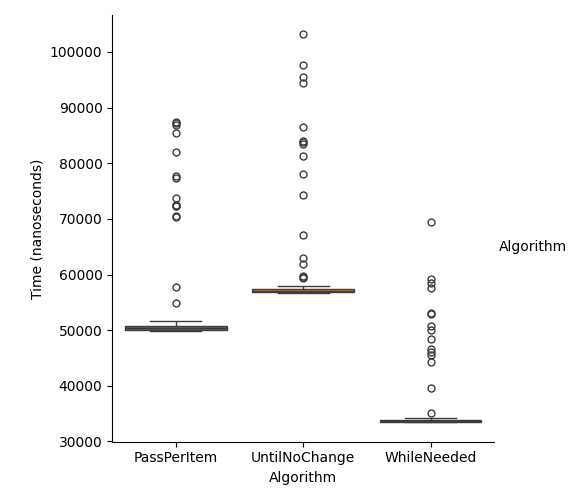
\includegraphics[width=\linewidth]{../figureIntDesc100.png}
    \caption{Size: 100}
    \label{fig:img1}
  \end{subfigure}
  \begin{subfigure}{0.3\textwidth}
    \centering
    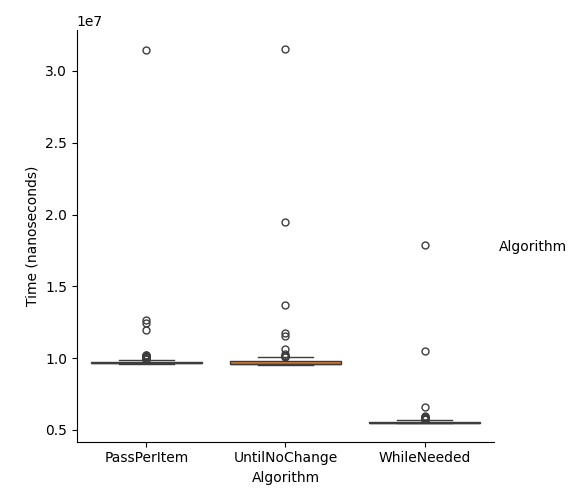
\includegraphics[width=\linewidth]{../figureIntDesc1000.png}
    \caption{Size 1000}
    \label{fig:img2}
  \end{subfigure}
  \begin{subfigure}{0.3\textwidth}
    \centering
    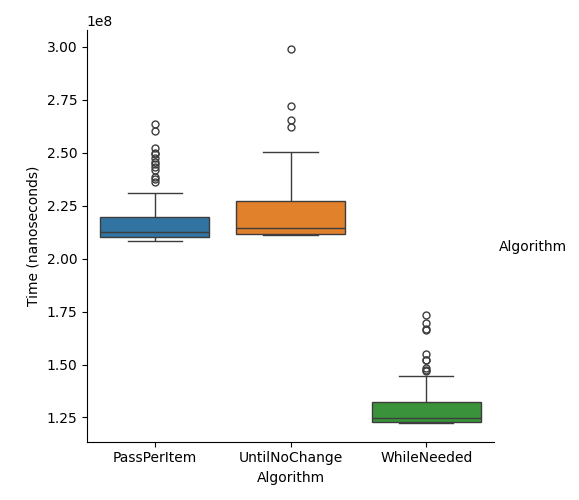
\includegraphics[width=\linewidth]{../figureIntDesc5000.png}
    \caption{Size 5000}
    \label{fig:img3}
  \end{subfigure}
  \caption{Time to sort descending arrays of Integers}
  \label{fig:three_images}
\end{figure}

\begin{figure}[ht]
  \centering
  \begin{subfigure}{0.3\textwidth}
    \centering
    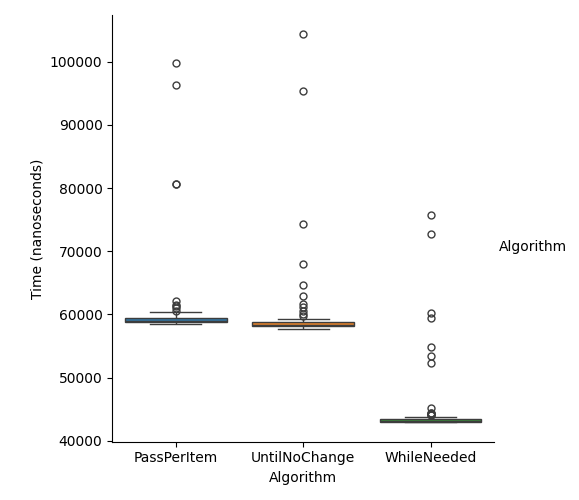
\includegraphics[width=\linewidth]{../figureByteDesc100.png}
    \caption{Size: 100}
    \label{fig:img1}
  \end{subfigure}
  \begin{subfigure}{0.3\textwidth}
    \centering
    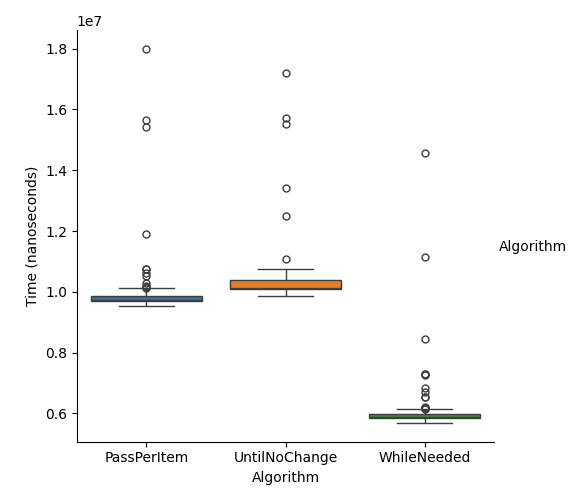
\includegraphics[width=\linewidth]{../figureByteDesc1000.png}
    \caption{Size 1000}
    \label{fig:img2}
  \end{subfigure}
  \begin{subfigure}{0.3\textwidth}
    \centering
    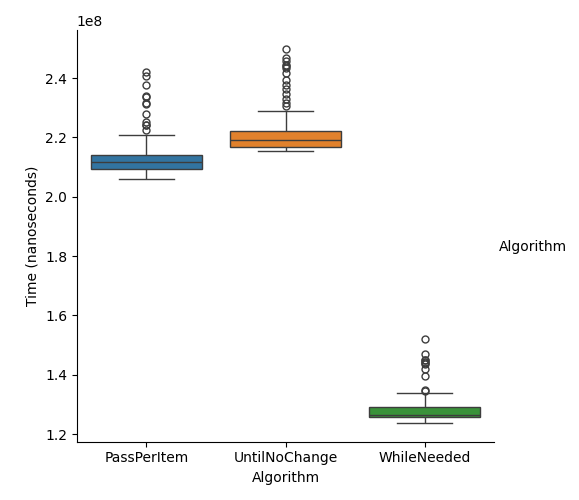
\includegraphics[width=\linewidth]{../figureByteDesc5000.png}
    \caption{Size 5000}
    \label{fig:img3}
  \end{subfigure}
  \caption{Time to sort descending array of Bytes}
  \label{fig:three_images}
\end{figure}

\begin{figure}[ht]
  \centering
  \begin{subfigure}{0.3\textwidth}
    \centering
    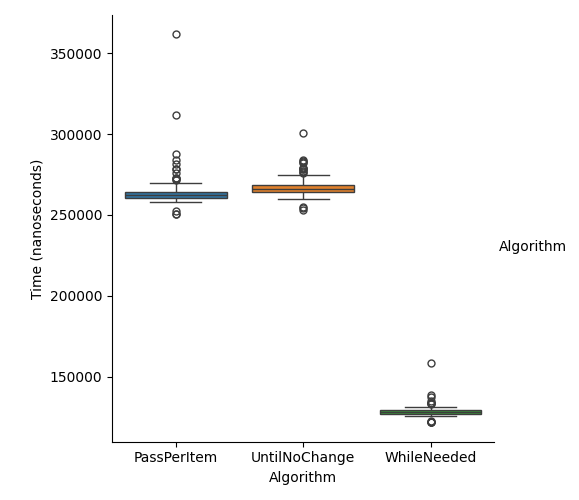
\includegraphics[width=\linewidth]{../figureStringDesc100.png}
    \caption{Size: 100}
    \label{fig:img1}
  \end{subfigure}
  \begin{subfigure}{0.3\textwidth}
    \centering
    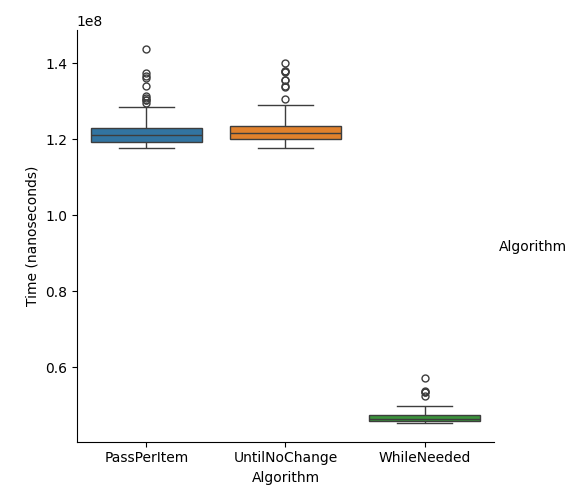
\includegraphics[width=\linewidth]{../figureStringDesc1000.png}
    \caption{Size 1000}
    \label{fig:img2}
  \end{subfigure}
  \begin{subfigure}{0.3\textwidth}
    \centering
    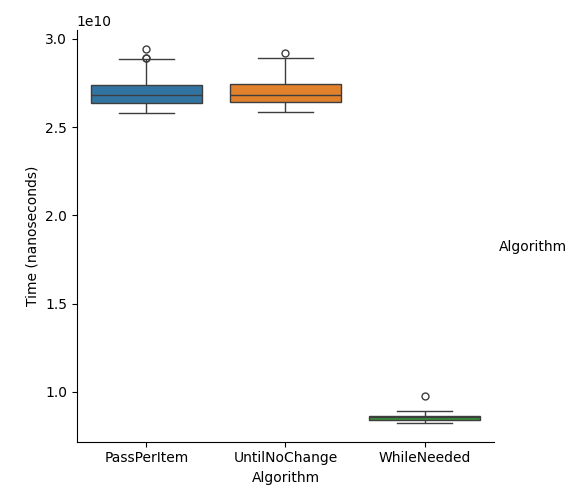
\includegraphics[width=\linewidth]{../figureStringDesc5000.png}
    \caption{Size 5000}
    \label{fig:img3}
  \end{subfigure}
  \caption{Time to sort descending array of String}
  \label{fig:three_images}
\end{figure}

\begin{figure}[ht]
  \centering
  \begin{subfigure}{0.3\textwidth}
    \centering
    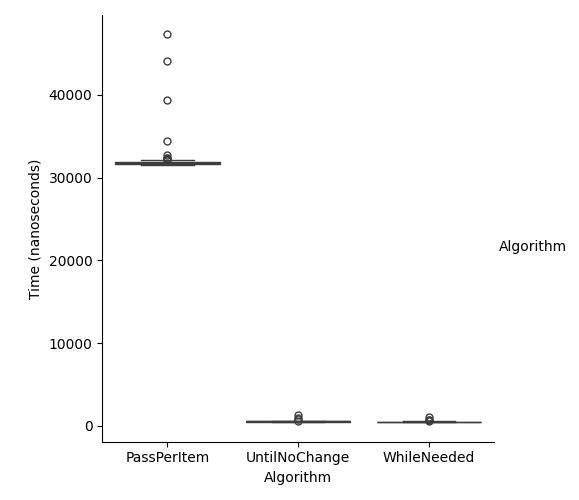
\includegraphics[width=\linewidth]{../figureIntAsc100.png}
    \caption{Size: 100}
    \label{fig:img1}
  \end{subfigure}
  \begin{subfigure}{0.3\textwidth}
    \centering
    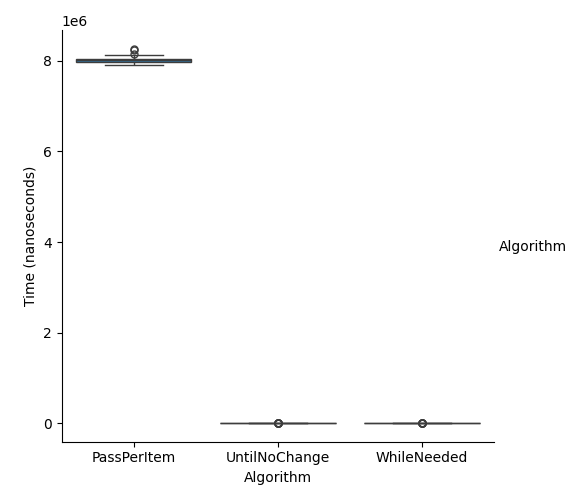
\includegraphics[width=\linewidth]{../figureIntAsc1000.png}
    \caption{Size 1000}
    \label{fig:img2}
  \end{subfigure}
  \begin{subfigure}{0.3\textwidth}
    \centering
    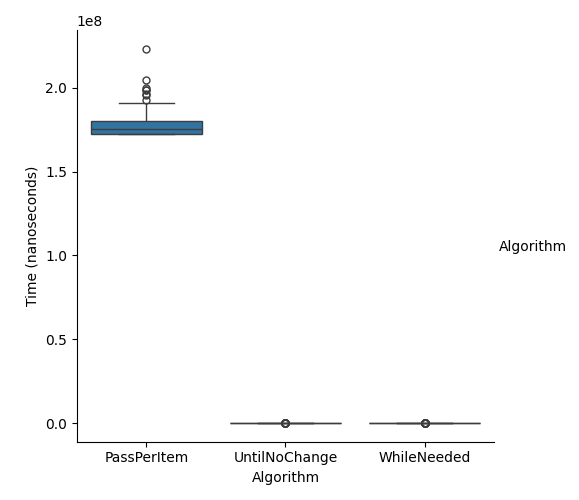
\includegraphics[width=\linewidth]{../figureIntAsc5000.png}
    \caption{Size 5000}
    \label{fig:img3}
  \end{subfigure}
  \caption{Time to sort ascending of random Integers}
  \label{fig:three_images}
\end{figure}

\begin{figure}[ht]
  \centering
  \begin{subfigure}{0.3\textwidth}
    \centering
    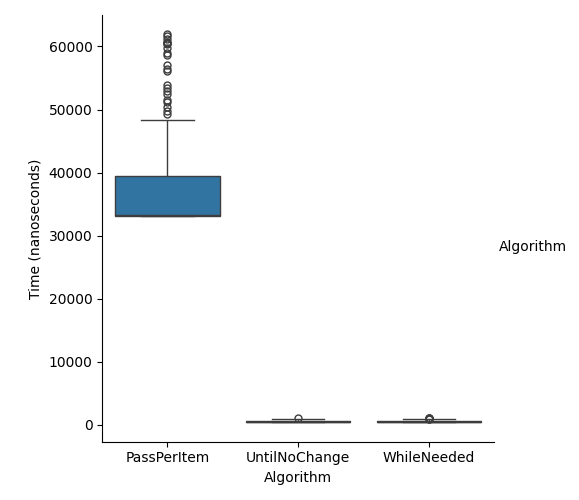
\includegraphics[width=\linewidth]{../figureByteAsc100.png}
    \caption{Size: 100}
    \label{fig:img1}
  \end{subfigure}
  \begin{subfigure}{0.3\textwidth}
    \centering
    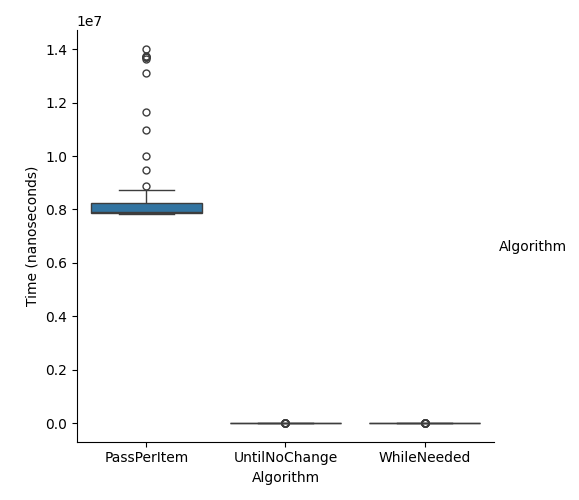
\includegraphics[width=\linewidth]{../figureByteAsc1000.png}
    \caption{Size 1000}
    \label{fig:img2}
  \end{subfigure}
  \begin{subfigure}{0.3\textwidth}
    \centering
    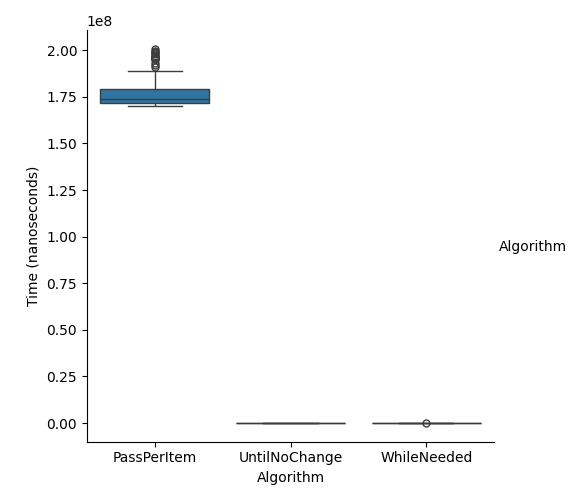
\includegraphics[width=\linewidth]{../figureByteAsc5000.png}
    \caption{Size 5000}
    \label{fig:img3}
  \end{subfigure}
  \caption{Time to sort ascending array of Bytes}
  \label{fig:three_images}
\end{figure}

\begin{figure}[ht]
  \centering
  \begin{subfigure}{0.3\textwidth}
    \centering
    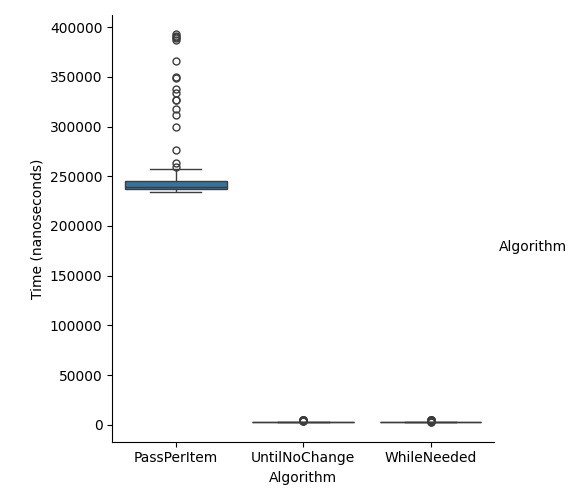
\includegraphics[width=\linewidth]{../figureStringAsc100.png}
    \caption{Size: 100}
    \label{fig:img1}
  \end{subfigure}
  \begin{subfigure}{0.3\textwidth}
    \centering
    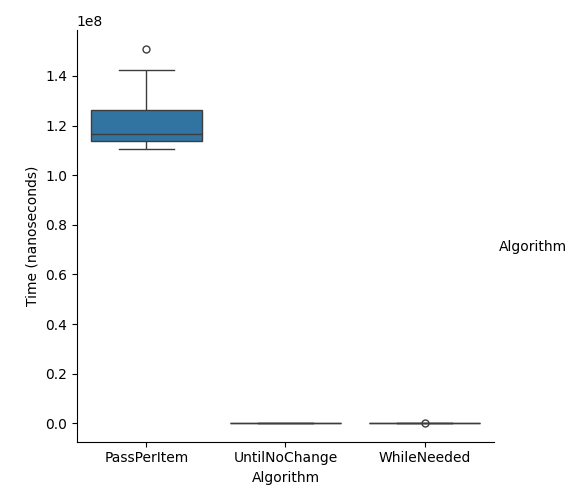
\includegraphics[width=\linewidth]{../figureStringAsc1000.png}
    \caption{Size 1000}
    \label{fig:img2}
  \end{subfigure}
  \begin{subfigure}{0.3\textwidth}
    \centering
    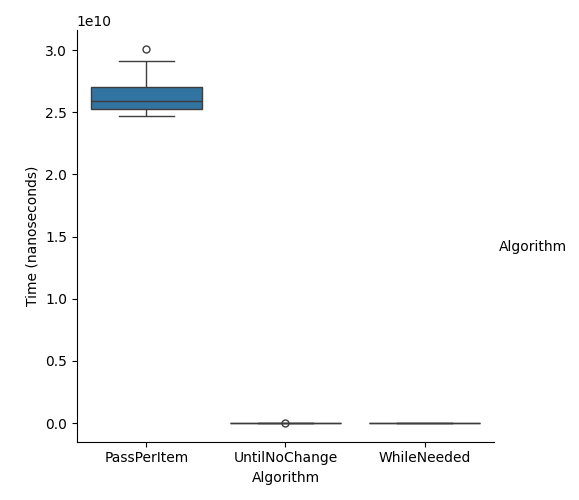
\includegraphics[width=\linewidth]{../figureStringAsc5000.png}
    \caption{Size 5000}
    \label{fig:img3}
  \end{subfigure}
  \caption{Time to sort ascending array of String}
  \label{fig:three_images}
\end{figure}

\end{document}
